%----------------------------------------------------------------------------------------
%	PACKAGES AND OTHER DOCUMENT CONFIGURATIONS
%----------------------------------------------------------------------------------------

\documentclass[DIV=calc, paper=a4, fontsize=11pt, twocolumn]{scrartcl}	 % A4 paper and 11pt font size

\usepackage{lipsum} % Used for inserting dummy 'Lorem ipsum' text into the template
\usepackage[english]{babel} % English language/hyphenation
\usepackage[protrusion=true,expansion=true]{microtype} % Better typography
\usepackage{amsmath,amsfonts,amsthm} % Math packages
\usepackage[svgnames]{xcolor} % Enabling colors by their 'svgnames'
\usepackage[hang, small,labelfont=bf,up,textfont=it,up]{caption} % Custom captions under/above floats in tables or figures
\usepackage{booktabs} % Horizontal rules in tables
\usepackage{fix-cm}	 % Custom font sizes - used for the initial letter in the document

\usepackage{sectsty} % Enables custom section titles
\allsectionsfont{\usefont{OT1}{phv}{b}{n}} % Change the font of all section commands

\usepackage{fancyhdr} % Needed to define custom headers/footers
\pagestyle{fancy} % Enables the custom headers/footers
\usepackage{lastpage} % Used to determine the number of pages in the document (for "Page X of Total")

\usepackage{graphicx}

\renewcommand{\headrulewidth}{0.0pt} % No header rule
\renewcommand{\footrulewidth}{0.0pt} % Thin footer rule

\usepackage{lettrine} % Package to accentuate the first letter of the text
\newcommand{\initial}[1]{ % Defines the command and style for the first letter
\lettrine[lines=2,lhang=0.1,nindent=0em]{
\color{DarkGoldenrod}
{\textsf{#1}}}{}}

%----------------------------------------------------------------------------------------
%	TITLE SECTION
%----------------------------------------------------------------------------------------

\usepackage{titling} % Allows custom title configuration

\newcommand{\HorRule}{\color{DarkGoldenrod} \rule{\linewidth}{1pt}} % Defines the gold horizontal rule around the title

\pretitle{\vspace{-2pt} \begin{flushleft} \HorRule \fontsize{30}{30} \usefont{OT1}{phv}{b}{n} \color{DarkRed} \selectfont} % Horizontal rule before the title

\title{Hunchkin} % Your article title

\posttitle{\par\end{flushleft}\vskip 0.5em} % Whitespace under the title

\preauthor{\begin{flushleft}\large \lineskip 0.5em \usefont{OT1}{phv}{b}{sl} \color{DarkRed}} % Author font configuration

\author{A recommendation platform} % Your name

\postauthor{\footnotesize \usefont{OT1}{phv}{m}{sl} \color{Black} % Configuration for the institution name
% Your institution

\par\end{flushleft}\HorRule} % Horizontal rule after the title

\date{} % Add a date here if you would like one to appear underneath the title block

%----------------------------------------------------------------------------------------

\begin{document}

\maketitle % Print the title

\thispagestyle{fancy} % Enabling the custom headers/footers for the first page 
\section*{}

\initial{Choice}
As with supermarket aisles that have give you a choice of different brands and flavors of chips, online retailers have flooded you with a wide choice of electronics, clothes, hotels etc. This tyranny of choice makes it difficult to find something that fits your needs and retailers, cognizant of this problem have approached it in many ways 

\initial{Recommendation}
Vendors like Amazon, Netflix and other retailers often use a technique called Collaborative Filtering which relies upon previous purchase history to recommend future purchases to their clients. While this method may provide greater accuracy with longer client history and frequently purchased products, when it comes to newer clients or products with less purchase history to rely upon, recommendations lose accuracy. Such is the case with high value items such as Jewelry and Electronics, and infrequent expenditures such as on leisure travel. 

\initial{Hunchkin}
Decision making for high value items or experiences is usually accomplished by combing through multiple information sources. Travel websites or online electric retailers may provide you the ability to sort by price, user reviews and possibly a few other atttributes and even offer you side-by-side comparisons along tens of features. But they rarely take into account your personal likings in the same way that Amazon and Netflix have tried to approach their recommendations. Recommendation systems can take a content-based filtering approach - the items characteristics are distilled down to a discrete set of features and attributes. Hunchkin does exactly that by modeling the domain for a product into a hierarchically organized set of discrete attributes and using information retrieval techniques to populate these attributes from the various data sources that the user typically uses. However, as noted, this hardly takes into consideration the particular buyer. Hunchkin uniquely combines the customer's "prior" beliefs - e.g. another product that she liked in the past - to narrow down to the attributes that are meaningful to this particular customer and come up with a set of recommendations. The elicitation of "priors" informs the entire short-listing and information display process. 

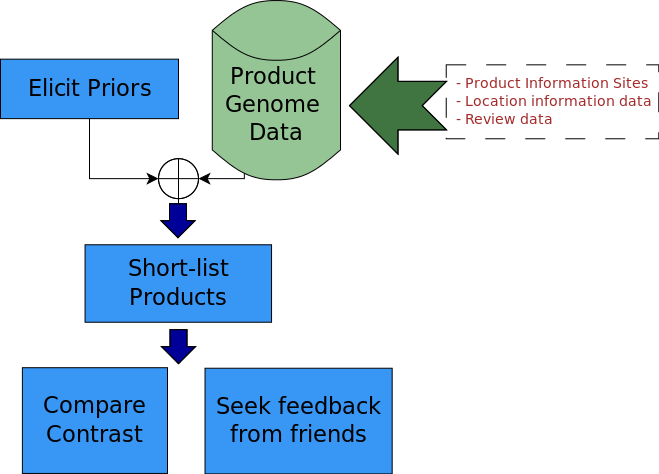
\includegraphics[height=80mm]{hk-concept.png}
A product "genome" represents the discrete attributes of the product. Distance functions at an aggregate level ("chromosome") are used to arrive at a vector similarity of the product with respect to the "priors". 

\par
There is an overwhelming amount of user feedback on products in blogs, specialized review sites (Trip Advisor, Yelp, for instance) and merchant websites. Reading hundreds of reviews and getting an overall picture is no longer easy. The problem is compounded by the ever-increasing review mills which generate a lot of "paid for" reviews on review sites. Hunchkin cuts through this problem by first, narrowing down the choices to a very small set that is customized for the buyer, as described before and then enabling the buyer to seek direct and pointed feedback about these products from her friends on her social networks. She is assured of reviews and feedback that she can trust more rather than an anonymous review, possibly written by someone who has been paid by the product manufacturer.

\section*{Hunchkin Hotels}

\initial{What it is }
Leisure travelers spend countless hours researching hotel features and reviews going back and forth between sites like Expedia, Kayak and Tripadvisor. When you travel alone for business, the decision variables are simple - location, wifi, dining etc. but family vacations can easily get complicated to research - activities for you and your partner, stuff for kids to do. Sometimes you can just go with a chain that you know but in many parts of the world, you really don't have that many chain hotels. The decision about which vacation hotel you pick is an important one because it can make or break a vacation. But it is not easy researching out all the information that you need to make this decision. It is further complicated by the huge volumes of reviews for popular hotels and also the increasing questionable quality of these hotels
\par
The product does the following:
\begin{itemize}
\item Asks you about a hotel that you liked in the past (could be from any location) during your hotel search along with dates of travel and destination
\item Gives you 5 recommendations which are similar to the hotel in features, amenities, dining, location etc.
\item Provides you with the ability to make detailed comparisons between these 5 hotels
\item You can ask your friends on Facebook or Google+ about opinions and recommendations from these 5 hotels
\end{itemize}

\subsection*{}

\initial{How it works }
Think of it as a Pandora for hotels. There is a genome that represents various aspects of a hotel - its features, the location, the services it provides, the dining and several others and this information is collected from various sources. There is a unique way of finding a "genome distance" between hotels and it finds hotels with the smallest distance (most similar to) from the hotel you say you liked. 

\subsection*{}

\initial{Revenue }
Hunchkin will initially rely primarily on affiliations with Online Travel Agencies (Expedia, Orbitz, Travelocity etc.) for referred sales commissions. Eventually as it establishes itself as a key Hotel search platform, advertising revenues will be added.


\subsection*{}

\initial{Competition }
Our competition will mainly be existing meta-search engines such as Kayak, Hipmunk etc. However, none of them have the recommendation capabilities that are in Hunchkin Hotels. 


\end{document}
